\begin{frame}[label=Fermat]
    \frametitle{Fermat}
    \begin{block}{Introduzione dell'infinitesimo}
        \begin{wrapfigure}{R}{0.3\textwidth}
            \centering
            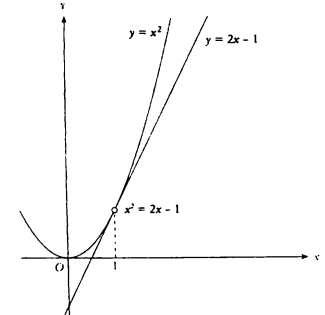
\includegraphics[width=0.25\textwidth]{Tangente-parabola.png}
        \end{wrapfigure}

        Fermat, intorno al 1630, ha già un suo metodo per trovare la tangente, 
        grazie ad un \textit{espediente algebrico}, 
        che divenne un concetto nuovo: \alert{l'infinitesimo}.
        \pause
        Cerchiamo il coefficiente angolare della retta tangente a una parabola
        $y = x^2$ nel punto $x=1$. Dato il punto $P_0=(1,1)$, che giace sulla curva 
        e ha ascissa $x=1$ si consideri 
        un punto \textit{infinitamente vicino ad esso}, che ha per ascissa $x=1+dx$
        (ove con $dx$ indichiamo appunto un \textit{infinitesimo}).
        L'ordinata sarà, secondo l'equazione data della parabola,
        $y= {(1+dx)}^2 = {1 + 2dx + {(dx)}^2}$.
        Il coefficiente angolare che congiunge questi due punti $P_0=(1,1)$ e 
        $P_1=(1+dx,{(1+dx)}^2)$ è dato dal rapporto fra le differenze fra le coordinate:
        \begin{center}
            $\frac{{(1+dx)}^2-1}{dx} = \frac{2dx+{(dx)}^2}{dx} = 2 + dx$
        \end{center}
        che è infinitamente vicino a 2. Sembra dunque ragionevole affermare che 
        il coefficiente angolare della tangente nel punto $P_0=(1,1)$ è $2$ e quindi 
        l'equazione della retta tangente in questo punto è
            $(y-1) = 2(x-1)$ , ovvero $y = 2x -1$
    \end{block}
\end{frame}